\begin{frame}{Placa de desarrollo utilizada para la interfaz}
	\centering
	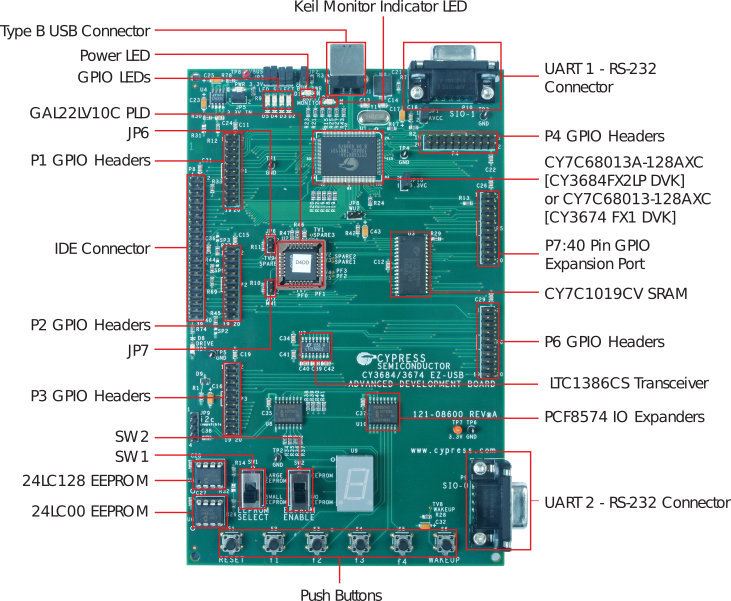
\includegraphics[height=0.8\textheight]{cy3684}
\end{frame}
\begin{frame}{El circuito integrado FX2LP}
	\centering
	\begin{tikzpicture}[scale=.58,>=latex]
		\begin{scope}[align=center,transform shape]
			\node	(aux1) {};
			\node[core,minimum height=95] (mis)	[left=of aux1,anchor=north east] {MIS};
			\node[core]	(ram) [right=of aux1,anchor=north west,text width=30] {16 kB RAM};
			\node[perif,text width=60] (xcvr) [left=of mis]	{Transceptor USB};
			\node[core,minimum size=60,text width=50] (uc) [above=of aux1] {8051 Mejorado};			
			\node[perif,node distance=2.9] (pll) [left=of uc] {PLL};
			\node	(aux2)	[right=of ram.south]{};				
			\node[core]	(bus)	[right=of aux2,rotate=90,anchor=north west]	{Bus de datos y direcciones};
			\node[perif]	(i2c)	[right=of bus.south east,anchor=north west]	{I2C};
			\node[perif]	(gpif)	[right=of bus.south west,anchor=south west] {GPIF};
			\node[perif,text width=40] (fifo) [below=of gpif] {4 kB FIFO};
			\node 			(aux3)	[right=of fifo]	{};
			\node 			(aux5) 	[left=of ram] {};
			\draw[<->]	(mis) -- (xcvr);
			\draw[<->]	(ram) -- (ram -| mis.east);
			\draw[<->]	(fifo) -- (fifo -| mis.east);
			\draw[<->]	(ram) to (ram -| bus.north);
			\draw[<->]	(uc) to (uc -| bus.north);
			\draw[<-]	(xcvr) to (xcvr |- pll.south);
			\draw[->]	(pll) to (uc);
			\draw[<->]	(i2c) to (i2c -| bus.south);
			\draw[<->]	(gpif) to (gpif -| bus.south);
			\draw[]		(fifo) -| (aux5.center);
		\end{scope}
		\begin{scope}[on background layer]
			\node[contenedor] (fx2) [fit=(pll)(xcvr)(uc)(bus)(mis)(ram)(fifo)(gpif)(i2c)(aux3)]{};
		\end{scope}
		\begin{scope}[transform shape]
			\node[text width=40,align=center]	(xtal)	[left=of pll]{Xtal \SI{24}{\mega\hertz}};
			\node	(host)	[left=3of xcvr]	{PC};
			\draw[<->,ultra thick] (host) -- node [above,text width=70,midway,align=center]{Comunicación USB} (xcvr);
			\draw[->] (xtal) to (pll);
			\draw[<->,ultra thick] (bus.240) -- node [above,align=center,text width=80] {Datos, direcciones y entradas adicionales}(bus.240 -| fx2.east);
			\draw[<->,thick] (gpif) to (gpif -| fx2.east);
			\draw[<->,thick] (fifo) to (fifo -| fx2.east);
			\draw[<->,thick] (i2c) to (i2c -| fx2.east);
		\end{scope}
	\end{tikzpicture}
\end{frame}
\begin{frame}{Configuración del dispositivo USB}
	\begin{columns}
		\begin{column}{.2\textwidth}
				\begin{tikzpicture}[scale=.32,align=center,>=latex]				\begin{scope}[node distance=0.4,transform shape]
						\node[buf]	(ep2b1)	[anchor=north]		{\ep{1}{2}{512}};
						\node[buf]	(ep2b2)	[below=of ep2b1]	{\ep{2}{2}{512}};
						\node[obuf]	(ep4b1) [below=of ep2b2]	{\ep{1}{4}{512}};
						\node[buf]	(ep4b2) [below=of ep4b1]	{\ep{2}{4}{512}};
						\node[obuf]	(ep6b1)	[below=of ep4b2]	{\ep{1}{6}{512}};
						\node[buf]	(ep6b2)	[below=of ep6b1]	{\ep{2}{6}{512}};
						\node[obuf]	(ep8b1)	[below=of ep6b2]	{\ep{1}{8}{512}};
						\node[buf]	(ep8b2)	[below=of ep8b1]	{\ep{2}{8}{512}};
					\end{scope}
				
					\begin{scope}[node distance=0.4, xshift=90,transform shape]
						\node[buf]	(ep2b3)	[anchor=north]		{\epg{1}{2}{1024}};
						\node[obuf] (ep2b4)	[below=of ep2b3]	{\epg{2}{2}{1024}};
						\node[obuf]	(ep2b5)	[below=of ep2b4]	{\epg{3}{2}{1024}};
						\node[obuf]	(ep8b3)	[below=of ep2b5]	{\ep{1}{8}{512}};
						\node[buf]	(ep8b4)	[below=of ep8b3]	{\ep{2}{8}{512}};
					\end{scope}
				
					\begin{scope}[on background layer,inner sep=1,rounded corners]
						\node[env, fit=(ep2b1)(ep2b2)]			(ep21)	{};
						\node[env, fit=(ep4b1)(ep4b2)]			(ep41)	{};
						\node[env, fit=(ep6b1)(ep6b2)]			(ep61)	{};
						\node[env, fit=(ep8b1)(ep8b2)]			(ep81)	{};
						\node[env, fit=(ep2b3)(ep2b4)(ep2b5)]	(ep22)	{};
						\node[env, fit=(ep8b3)(ep8b4)]			(ep82)	{};
					\end{scope}
				
					\begin{scope}[]
						\node[draw=black,inner sep=2,fit=(ep21)(ep82)](marco){};
					\end{scope}
					\begin{scope}[transform shape,node distance=2.5]
						\draw (marco.north) to (marco.south);
						\node[left=of ep2b1.north east,anchor=north east](add1)	{0xF000};
						\node[left=of ep2b1.south east,anchor=south east](add2)	{0xF1FF};
						\node[left=of ep2b2.north east,anchor=north east](add3)	{0xF200};
						\node[left=of ep4b1.north east,anchor=north east](add4)	{0xF400};
						\node[left=of ep6b1.north east,anchor=north east](add5)	{0xF800};
						\node[left=of ep8b1.north east,anchor=north east](add6)	{0xFC00};
						\node[left=of ep8b2.south east,anchor=south east](add7)	{0xFFFF};
						\draw[dashed] (add1.north west) to (add1.north west -| marco.east);
						\draw[dashed] (add3.north west) to (add3.north west -| ep21.east);
						\draw[dashed] (add4.north west) to (add4.north west -| marco.east);
						\draw[dashed] (add5.north west) to (add5.north west -| marco.east);
						\draw[dashed] (add6.north west) to (add6.north west -| marco.east);
						\draw[dashed] (add7.south west) to (add7.south west -| marco.east);
					\end{scope}
				\end{tikzpicture}
		\end{column}
		\begin{column}{.7\textwidth}
			La configuración de las tuberías de comunicación se definieron con la finalidad de obtener el mayor ancho de banda posible a la entrada.
			\begin{itemize}
				\only<1>{\item Entrada:
					\begin{itemize}
						\item Extremo EP2
						\item Transferencias Isocrónicas
						\item 1024 Bytes máximo por transferencia
						\item 3 Buffers
					\end{itemize}}
				\only<2>{\item Salida:
					\begin{itemize}
						\item Extremo EP8
						\item Transferencia por bultos
						\item 512 Butes por transferencia
						\item 2 Buffers
					\end{itemize}}
			\end{itemize}
		\end{column}
	\end{columns}
\end{frame}
%\begin{frame}{Cypress Software Development Kit}
%	\begin{columns}
%		\begin{column}{.2\textwidth}
%			\begin{tikzpicture}[scale=.42]
%				\begin{scope}[transform shape,node distance=1,>=latex]
%					\node[mealy]	(start)	[]	{Iniciar: Reset \\ \verb~main();~ };
%					\node[moore]	(init)	[below=of start]	{Inicia Variables de Estado}
%						edge[<-,thick] (start);
%					\node[moore]	(us1)	[below=of init]		{ \verb~TD\_Init();~ }
%						edge[<-,thick]	(init);
%					\node[moore]	(EI)	[below=of us1]	{Habilita\\Interrupciones}
%						edge[<-,thick](us1);
%					\node[node distance=0.7]			(aux1)	[below=of EI] 	{};
%					\draw[<-,thick](aux1.base) to (EI);
%					\node[moore,node distance=.5]	(poll)	[below=of aux1]	{\verb~TD\_Poll();~ }
%						edge[<-,thick](aux1.base);
%					\node[ask]		(pr1)	[below=of poll]	{Paquete de Setup}
%						edge[<-,thick](poll);
%					\node[moore]	(setup)	[right=of pr1]	{\verb~SetupComand();~ };
%					\draw[->,thick] (setup) |- (aux1.base);
%					\node[]			(aux2)	[below=of pr1]	{};
%					\draw[->,thick]	(pr1) -- node[above,near start]{Si} (setup);
%					\draw[thick]	(pr1) -- node[left,near start]{No}	(aux2.base);
%					\node[node distance=2.5](aux3)	[left=of aux2] {};
%					\draw[thick]	(aux2.base) -- (aux3.base);
%					\draw[->,thick]	(aux3.base)	|-	(aux1.base);
%				\end{scope}
%			\end{tikzpicture}
%		\end{column}
%		\begin{column}{.6\textwidth}
%			\begin{itemize}
%				\item El programa inicia al comienzo del main();
%				\item Inicia todas las variables de estado
%				\item TD\_Init ejecuta la configuración del usuario
%				\item El usuario debe configurar las interrupciones que desea habilitar. Al salir de TD\_Init, el programa habilita todas (\verb~EA=1~)
%				\item Finalmente, se ejecuta las instrucciones que el usuario programa de manera específica
%				\item Además, se ejecutan las funciones que controlan el USB.
%			\end{itemize}
%		\end{column}
%	\end{columns}
%\end{frame}
